\documentclass[11pt]{article}
\usepackage[utf8]{inputenc}
\usepackage{graphicx}

\begin{document}

\begin{figure}[!ht]
    \title{Nova Methodi \\
    \large Ex evolutione methodorum nostrarum productiva veniet.}
    \author{Luís Kaldwin A.S}
    \maketitle
    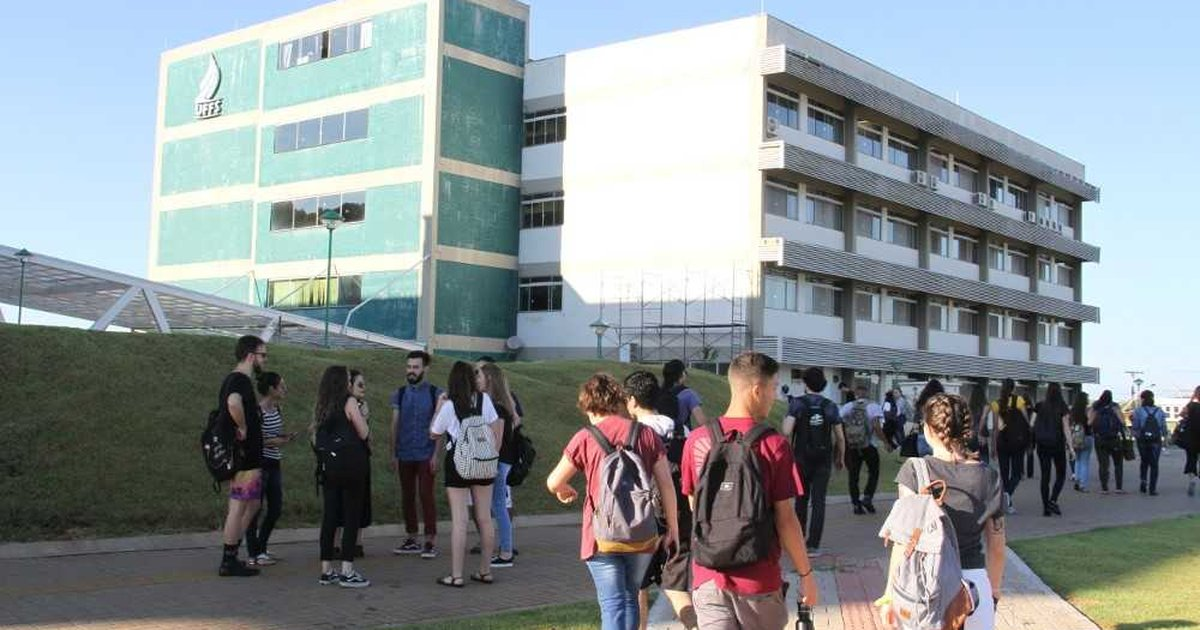
\includegraphics[width=\linewidth]{cover.jpg} 
    \caption{Universidade Federal da Fronteira Sul.}
    \label{fig:cover}
\end{figure}
\pagebreak

\section{Introductio ad \LaTeX}
From now on, the plan is to use \LaTeX\ to write notes and documents related to 
university work, classes and research, if that ever is within the range of opportunity. \\
Below, you will find a simple example of the workings of \LaTeX\ in a simple document and a small 
inquiry of why I might be using it. 
\\

A rectangle has side lengths of $(x+1)$ and $(x+3)$. \\
The equation gives the area of the rectangle. \\
\[A(x) = x^2 + 4x + 3\]

\end{document}